%% State Space Modelling of Dynamic Systems
%% Lecture 20: State Feedback Control
\def\FileDate{10/02/02}
\def\FileVersion{1.0}
% ----------------------------------------------------------------
% Notes pages *********************************************************
% ----------------------------------------------------------------

\begin{slide}
   \heading{State Feedback Control}
One of the advantages of state space models is that it is possible to apply state feedback to place the closed loop poles into any desired positions.

\textbf{State Space Design Methodology}

\begin{enumerate}
	\item Design control law to place closed loop poles where desired
	\item If full state not available for feedback, then design an \emph{Observer} to compute the states from the system output
	\item Combine \emph{Observer} and \emph{Controller} -- this takes the place of the \emph{Classical Compensator}
	\item Introduce the \emph{Reference Input} -- affects the closed loop zeros but not the poles making it possible to improve the transient response and tracking accuracy
\end{enumerate}	
\end{slide}

\begin{slide}
   \heading{State Feedback Compensator}
   \begin{center}
   	\resizebox{280pt}{!}{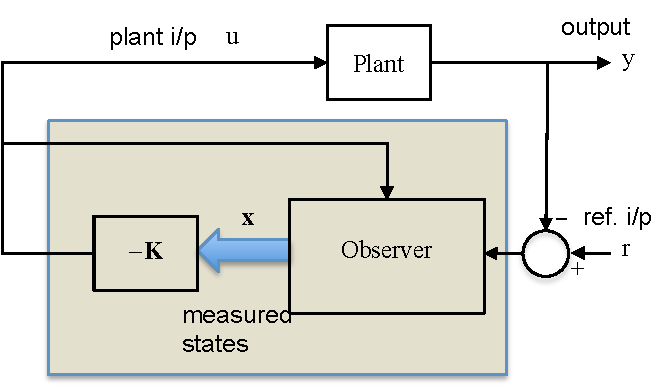
\includegraphics{pictures/statefb.pdf}}
   \end{center}
\end{slide}

\section*{Finding the Control Law} % (fold)
\label{sec:finding_the_control_law}

We shall only consider SISO systems here.

Let the input to the plant, $u$ be derived from the reference input $r$, and the states, $\mathbf{x}$, as follows:
\[
u=r-\mathbf{Kx}=r-(k_1x_1+k_2x_2+\cdots k_nx_n)
\]
Thus:
\begin{eqnarray*}
	\dot{\mathbf{x}} & = & \mathbf{Ax}+\mathbf{B}u \\
	                 & = & \mathbf{Ax}+\mathbf{B}(r = \mathbf{Kx}) \\
	                 & = & \mathbf{Ax}+\mathbf{B}u \\	
\end{eqnarray*} 

The state matrix for the closed loop system with input, $r$,  is:  $\mathbf{A}-\mathbf{BK}$ and taking Laplace Transforms  (ignoring initial conditions) gives:
\[
	s\mathbf{X}(s) = (\mathbf{A}-\mathbf{BK})\mathbf{X}(s) + \mathbf{B}R(s)
\]
Therefore 
\[
    (s\mathbf{I}-\mathbf{A}+\mathbf{BK})\mathbf{X}(s) = \mathbf{B}R(s).
\]

The closed loop poles are the roots of $s$ in the Characteristic Equation (CE):
\begin{equation}
	\label{eq:1}
	\det\left[s\mathbf{I}-\mathbf{A}+\mathbf{BK}\right]=0
\end{equation}
 
Suppose the desired closed loop poles are to be at $p_1$, $p_2$, $\cdots$, $p_n$, then the desired CE is:
\begin{equation}
	\label{eq:2}
	\alpha_c(s) = (s-p_1)(s-p_2)\cdots(s-p_n)=0
\end{equation} 

Equation (\ref{eq:2}) is multiplied out to a polynomial in $s$.

Finally, we need to find the $k$  coefficients in $\mathbf{K}$ such that the polynomials in equations  (\ref{eq:1})  and  \ref{eq:2}) above have matching coefficients in each power of $s$.

This leads to a set of linear equations in the $k$'s  which can always be solved to give the required feedback control law, for whatever closed loop pole locations are given.

\subsection*{Example 1} % (fold)
\label{sub:example_1}

\textbf{Problem}: Given,
\[
{\bf{\dot x}} = \left[ {\begin{array}{*{20}c}
   { - 4} & 0  \\
   0 & { - 11}  \\
\end{array}} \right]{\bf{x}} + \left[ {\begin{array}{*{20}c}
   1  \\
   { - 1}  \\
\end{array}} \right]u
\]
find the feedback control law which places the closed-loop poles at: $-10\pm j10$.

\textbf{SOLUTION}:
\begin{eqnarray*}
	0 & = & \det \left[ {s{\bf{I}} - {\bf{A}} + {\bf{BK}}} \right] = \det \left\{ {\left. {\left[ {\begin{array}{*{20}c}
	   {s + 4} & 0  \\
	   0 & {s + 11}  \\
	\end{array}} \right] + \left[ {\begin{array}{*{20}c}
	   1  \\
	   { - 1}  \\
	\end{array}} \right]\left[ {\begin{array}{*{20}c}
	   {k_1 } & {k_2 }  \\
	\end{array}} \right]} \right\}} \right. \\
	0 & = & \det \left[ {\begin{array}{*{20}c}
	   {s + 4 + k_1 } & {k_2 }  \\
	   { - k_1 } & {s + 11 - k_2 }  \\
	\end{array}} \right] \\
	0 & = & (s + 4 + k_1 )(s + 11 - k_2 ) - (k_2 )( - k_1 ) \\
	0 & = & (s+4+k_1)(s+11-k_2)+k_1k_2
\end{eqnarray*}
\begin{equation}
	\label{eq:3}
	s^2+(15+k_1-k_2)s+(44+11k_1-4k_2)=0
\end{equation}

Now the desired CE is:
\[
\alpha_c(s)=(s+10-j10)(s+10-j10) = 0
\]
\begin{equation}\label{eq:4}
	s^2+20s+200=0
\end{equation}

Therefore matching coefficients in Eqs. (\ref{eq:3}) and (\ref{eq:4}):
\[
\begin{array}{c}
 s^2 :1 = 1 \to {\rm{OK}} \\ 
 s^1 :15 + k_1  - k_2  = 20 \to k_1  - k_2  = 5 \\ 
 s^0 :44 + 11k_1  - 4k_2  = 200 \to 11k_1  - 4k_2  = 156 \\ 
 \end{array}
\]

 

Solving for the $k$'s:
\[
\left[ {\begin{array}{*{20}c}
   1 & { - 1}  \\
   {11} & { - 4}  \\
\end{array}} \right]\left[ {\begin{array}{*{20}c}
   {k_1 }  \\
   {k_2 }  \\
\end{array}} \right] = \left[ {\begin{array}{*{20}c}
   5  \\
   {156}  \\
\end{array}} \right]
\]
% MathType!MTEF!2!1!+-
% faaagaart1ev2aaaKnaaaaWenf2ys9wBH5garuavP1wzZbqedmvETj
% 2BSbqefm0B1jxALjharqqtubsr4rNCHbGeaGqiVu0Je9sqqrpepC0x
% bbL8FesqqrFfpeea0xe9Lq-Jc9vqaqpepm0xbba9pwe9Q8fs0-yqaq
% pepae9pg0FirpepeKkFr0xfr-xfr-xb9Gqpi0dc9adbaqaaeGaciGa
% aiaabeqaamaabaabaaGcbaWaamWaaeaafaWabeGabaaabaGaam4Aam
% aaBaaaleaacaaIXaaabeaaaOqaaiaadUgadaWgaaWcbaGaaGOmaaqa
% baaaaaGccaGLBbGaayzxaaGaeyypa0ZaaSaaaeaacaaIXaaabaGaey
% OeI0IaaGinaiabgUcaRiaaigdacaaIXaaaamaadmaabaqbamqabiGa
% aaqaaiabgkHiTiaaisdaaeaacaaIXaaabaGaeyOeI0IaaGymaiaaig
% daaeaacaaIXaaaaaGaay5waiaaw2faamaadmaabaqbamqabiqaaaqa
% aiaaiwdaaeaacaaIXaGaaGynaiaaiAdaaaaacaGLBbGaayzxaaGaey
% ypa0ZaaSaaaeaacaaIXaaabaGaaG4naaaadaWadaqaauaadeqaceaa
% aeaacaaIXaGaaG4maiaaiAdaaeaacaaIXaGaaGimaiaaigdaaaaaca
% GLBbGaayzxaaGaeyypa0ZaamWaaeaafaWabeGabaaabaGaaGymaiaa
% iMdacaGGUaGaaGinaiaaiMdacaaIYaGaaGyoaaqaaiaaigdacaaI0a
% GaaiOlaiaaisdacaaIYaGaaGyoaaaaaiaawUfacaGLDbaaaaa!5BC6!
\[
\left[ {\begin{array}{*{20}c}
   {k_1 }  \\
   {k_2 }  \\
\end{array}} \right] = \frac{1}{{ - 4 + 11}}\left[ {\begin{array}{*{20}c}
   { - 4} & 1  \\
   { - 11} & 1  \\
\end{array}} \right]\left[ {\begin{array}{*{20}c}
   5  \\
   {156}  \\
\end{array}} \right] = \frac{1}{7}\left[ {\begin{array}{*{20}c}
   {136}  \\
   {101}  \\
\end{array}} \right] = \left[ {\begin{array}{*{20}c}
   {19.429}  \\
   {14.429}  \\
\end{array}} \right]
\]

 

Therefore the required feedback control law is:
% MathType!MTEF!2!1!+-
% faaagaart1ev2aaaKnaaaaWenf2ys9wBH5garuavP1wzZbqedmvETj
% 2BSbqefm0B1jxALjharqqtubsr4rNCHbGeaGqiVu0Je9sqqrpepC0x
% bbL8FesqqrFfpeea0xe9Lq-Jc9vqaqpepm0xbba9pwe9Q8fs0-yqaq
% pepae9pg0FirpepeKkFr0xfr-xfr-xb9Gqpi0dc9adbaqaaeGaciGa
% aiaabeqaamaabaabaaGcbaGaamyDaiabg2da9iaadkhacqGHsislda
% WadaqaauaadeqabiaaaeaacaaIXaGaaGyoaiaac6cacaaI0aGaaGOm
% aiaaiMdaaeaacaaIXaGaaGinaiaac6cacaaI0aGaaGOmaiaaiMdaaa
% aacaGLBbGaayzxaaGaaCiEaaaa!3DCD!
\[
u = r - \left[ {\begin{array}{*{20}c}
   {19.429} & {14.429}  \\
\end{array}} \right]{\bf{x}}
\]



\textbf{COMMENT}
This matching of coefficients can always be done, though it is tedious for $n>3$, \textbf{EXCEPT} in the case of the \emph{Control Canonical Form}.

% subsection example_1 (end)
 
% section finding_the_control_law (end)

\section{State Feedback in the Case of the Control Canonical Form} % (fold)
\label{sec:state_feedback_in_the_case_of_the_control_canonical_form}


In the control canonical form we have matrices:

 
with open loop CE:
 
Feedback results in the closed loop CE:
 

   1)
 
Suppose the desired CE is:

 

or         2)

Matching coefficients in equns 1)  &  2)  is now simple:

 


 
eg.Given the system TF:
 
find the control law for the control canonical form which places the closed loop poles at s=−10±10j.
Answer:
 
The control canonical form has matrices:
 
NB:  C  is obtained from the TF numerator   (0s+7)
so:    
and the closed loop CE is :
        1)
The desired CE is:
 
Comparing equns  1)  and  2) gives:
 
giving the control law as:   


% section state_feedback_in_the_case_of_the_control_canonical_form (end)



%----------------------------------------------------------------
% The end of notes
% ----------------------------------------------------------------
\endinput

%%% Local Variables: 
%%% mode: latex
%%% TeX-master: t
%%% End: 
